\chapter{Empirical Results}\label{chap:mainresults}
\todo{chapter intro} The approach usually starts with the problem definition and continues with what you have done. Try to give an intuition first and describe everything with words and then be more formal like `Let $g$ be ...'.

Start with a very short motivation why this is important. Then, as stated above, describe the problem with words before getting formal.
\section{Database}

The data used for this study is from the tick-by-tick Trade and Quote database traded at the NYSE. As \citet{hausman1992} use one-year data for their analysis, we also take the full trading sample of IBM stock on NYSE from January 3 to December 29 of 2023 for the descriptive statistics and market microstructure analysis parts. For the forecasting analysis, the first 10 months of 2023 will be used for in-sample forecasting, and the last 2 months will be left for the out-of-sample forecasting.

Before arriving at the final dataset, we first match the trade and quote databases. Since the resolution of the current NYSE database is at nanosecond, we simply backward match the trade to the prevailing quote. We only use the data within the regular trading hours (9:30:00–16:00:00) and do not take into account overnight trading. The transactions happening at the first-second of each trading day are removed to reduce contamination from the opening call at the stock exchange. \tabref{tab:table-2} summarizes the number of observations used:

\begin{table}[ht]
\centering
\small
\renewcommand{\arraystretch}{1.3} % Increases row height
\setlength{\tabcolsep}{10pt} % Increases column separation
\resizebox{\textwidth}{!}{%
\begin{tabular}{|c|l|c|}
\hline
\textbf{Purpose}       & \multicolumn{1}{c|}{\textbf{Timeframe}} & \textbf{Number of transactions} \\ \hline
Panel A: Total         & January 3 - December 29, 2023           & 1,905,393                       \\ \hline
Panel B: In-sample     & January 3 - October 31, 2023            & 1,641,694 (86\% of total sample) \\ \hline
Panel B: Out-of-sample & November 1 - December 29, 2023          & 263,699 (14\% of total sample)   \\ \hline
\end{tabular}%
}
\caption{Summary of Database: IBM traded on NYSE, 2023}
\label{tab:table-2}
\end{table}


\section{Descriptive Statistics (Full Sample)}

{\noindent\bfseries Price Change }
\begin{table}[htbp]
\centering
\begin{tabular}{ll}
\toprule
\textbf{Statistic} & \textbf{IBM}\\
\midrule
\textbf{\% trades at prices:} & \\
> Midquote & 40.07\\
= Midquote & 16.65\\
< Midquote & 43.28\\
\textbf{Price change, $Z_k$} & \\
Mean & 0.0000\\
Std. dev. & 0.0134\\
\bottomrule
\end{tabular}
\caption{Summary statistics: Price Changes}
\label{tab:3}
\end{table}

\begin{figure}[htbp]
    \centering
    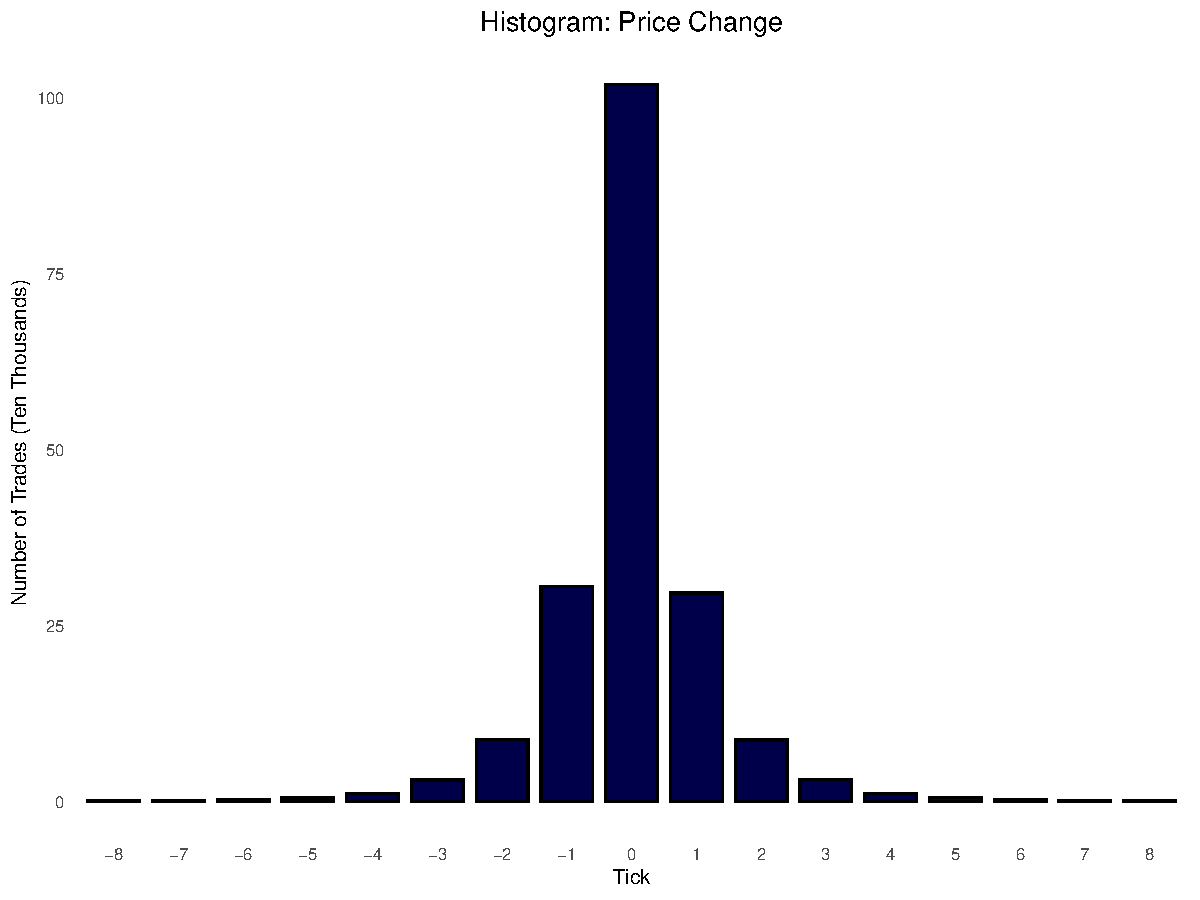
\includegraphics[width=0.8\textwidth]{figures/descriptive stat/price_change_IBM_N_2023.pdf}
    \caption{Histogram of Price Changes: IBM on NYSE, 2023}
    \label{fig:price-change-2023}
\end{figure}


\section{Panel A: Market Microstructure Analysis}

\section{Panel B: Forecasting Analysis}